\documentclass[twoside]{article}
\usepackage{amsgen,amsmath,amstext,amsbsy,amsopn,amssymb,}
\usepackage{graphicx}
\usepackage{epsfig}

\setlength{\oddsidemargin}{0.1 in} \setlength{\evensidemargin}{-0.1
in} \setlength{\topmargin}{-0.6 in} \setlength{\textwidth}{6.5 in}
\setlength{\textheight}{10.4 in} \setlength{\headsep}{0.1 in}
\setlength{\parindent}{0 in} \setlength{\parskip}{0.1 in}

\newcommand{\homework}[2]{
   \pagestyle{myheadings}
   \thispagestyle{plain}
   \newpage
   \setcounter{page}{1}
   \noindent
   \begin{center}
   \framebox{
      \vbox{\vspace{2mm}
       \hbox to 6.28in { {\bf Math 1700:~Elementary Statistics \hfill} }
       \vspace{6mm}
       \hbox to 6.28in { {\Large \hfill #1 (#2)  \hfill} }
       \vspace{6mm}
      \vspace{2mm}}
   }
   \end{center}
   \markboth{#1}{#1}
   \vspace*{4mm}
}

\newcommand{\bbF}{\mathbb{F}}
\newcommand{\bbX}{\mathbb{X}}
\newcommand{\bI}{\mathbf{I}}
\newcommand{\bX}{\mathbf{X}}
\newcommand{\bY}{\mathbf{Y}}
\newcommand{\bepsilon}{\boldsymbol{\epsilon}}
\newcommand{\balpha}{\boldsymbol{\alpha}}
\newcommand{\bbeta}{\boldsymbol{\beta}}
\newcommand{\0}{\mathbf{0}}

\begin{document}

\homework{$4^{th}$ Week Summary}{09/17/25}
\vspace{-.3in}
\begin{itemize}
\item \textbf{Random Variables}: A variable that assumes a unique numerical value for each of the outcomes
\subitem \textbf{Discrete}: A random variable that can assume a countable number of values
\subitem \textbf{Continuous}: A random variable that can assume an uncountable (continuum) number of values
\item \textbf{Probability function}: A distribution of the probabilities associated with each of the values of a random variable
\item \textbf{Probability distribution}: A rule, $P(x)$, that assigns probabilities to the values of the random variables
\subitem Property 1: $0\leq P(x)\leq 1$
\subitem Property 2: $\sum_\textrm{all\ x}P(x)=1$
\item \textbf{Population Parameters}
\subitem $\mu = \sum_{i=1}^n x_i P(x_i)$ is the population mean.
\subitem $\sigma^2 = \sum_{i=1}^n (x_i-\mu)^2 P(x_i) = \sum_{i=1}^n [x_i^2 P(x_i)] - \mu^2$ \ is the population variance
\subitem $\sigma = \sqrt{\sigma^2}$ \ is the population standard deviation.
\item \textbf{Binomial probability experiment}:
\subitem 1. There are $n$ repeated identical independent trials.
\subitem 2. Each trial has two possible outcomes (\textit{success} or \textit{failure}).
\subitem 3. $P(\mathrm{success})=p$, $P(\mathrm{failure})=q$, and $p+q=1$.
\subitem 4. The binomial random variable $x$ is the count of the number of successful trials that occur; $x$ \ may take on any integer value from zero to $n$
\item \textbf{Binomial probability function}: 
\item $P(x) = \dfrac{n!}{x! (n-x)!}(p^x)(q^{n-x})$, \ \ \ for $x = 0, 1, 2, \cdots, n$
\subitem $\mu=np$
\subitem $\sigma^2=npq$
\subitem $\sigma=\sqrt{npq}$

\begin{figure}[h]
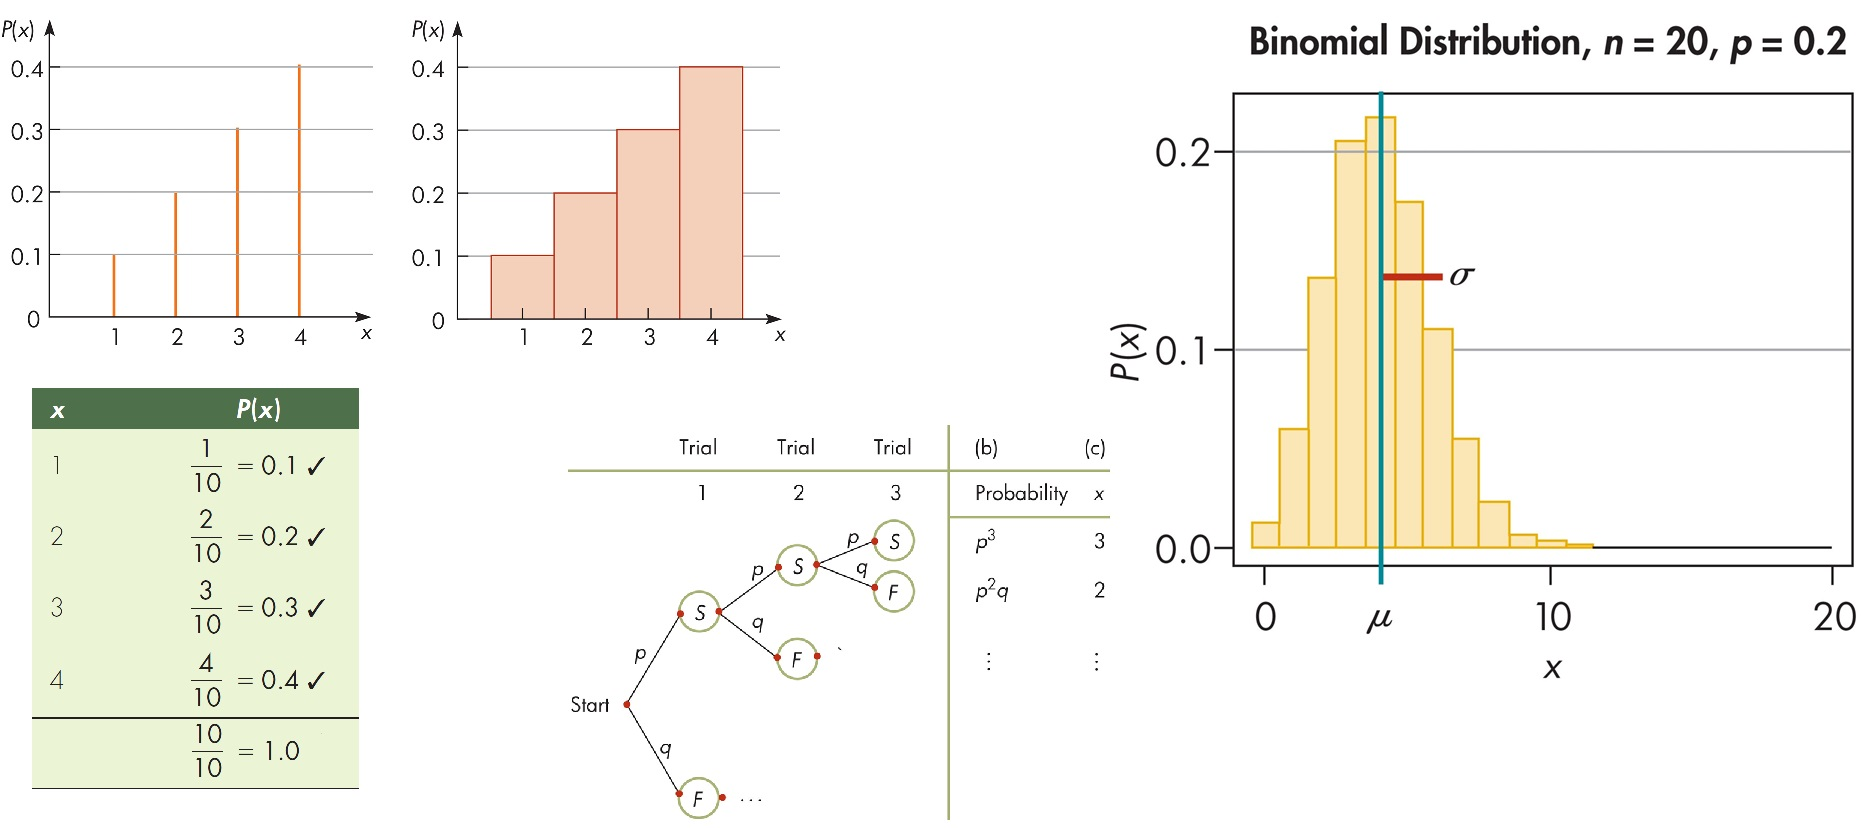
\includegraphics[angle=0,width=\textwidth] {graphs5.jpg}
\end{figure}
\end{itemize}
\end{document}
